\documentclass[sigplan,10pt,anonymous,review]{acmart}
\settopmatter{printfolios=true,printccs=false,printacmref=false}

\usepackage[utf8]{inputenc}
\usepackage{url}
\usepackage{amsmath}
\usepackage{mathbbol}
\usepackage{mathtools}
\usepackage{hyperref}

% Two column itemize
\usepackage{multicol}

% Example code
\usepackage{listings}

% Diagrams
\usepackage{tikz}

% Mathbb doesn't support digits
\usepackage{bbm}

% inference rules
\usepackage{mathpartir}

% Newline inside table
\usepackage{makecell}

% Fix autoref's example treatment 
\newtheorem{example}{Example}
\newcommand{\exampleautorefname}{Example}
\newcommand{\nitheoremautorefname}{Theorem}
\newcommand{\nidefinitionautorefname}{Definition}

% Do not use italics in definitions and theorems
\theoremstyle{definition}
\newtheorem{nidefinition}{Definition}
\newtheorem{nitheorem}{Theorem}
\newtheorem{nilemma}{Lemma}
\renewcommand{\sectionautorefname}{\S}%
\renewcommand{\subsectionautorefname}{\S}%

% Abbreviations
\newcommand{\lambdacalc}{$\lambda$-calculus}
\newcommand{\picalc}{$\pi$-calculus}
\newcommand{\Picalc}{$\pi$-Calculus}

% Typing rules
\newcommand{\stacked}[1]{\mprset{flushleft} \inferrule*{}{#1}}
\newcommand{\datatype}[2]{{\mprset{fraction={===}} \inferrule{#1}{#2}}}

\newcommand{\type}[1]{\textcolor{blue}{\operatorname{#1}}}
\newcommand{\constr}[1]{\textcolor{orange}{\operatorname{#1}}}
\newcommand{\func}[1]{\textcolor{olive}{\operatorname{#1}}}

% Constructors
\newcommand{\PO}{\constr{\mathbb{0}}}
\newcommand{\comp}[2]{#1 \, \constr{\parallel} \, #2}
\newcommand{\new}{\constr{\boldsymbol{\nu}} \,}
\newcommand{\send}[2]{#1 \, \constr{\langle} \, #2 \,\constr{\rangle} \,}
\newcommand{\recv}[2]{#1 \, \constr{\mathbb{(}} \, #2 \, \constr{\mathbb{)}} \,}
\newcommand{\suc}{\constr{\scriptstyle 1+}}
\newcommand{\unit}{\constr{\mathbbm{1}}}
\newcommand{\base}[1]{\constr{B[} \, #1 \, \constr{]}}
\newcommand{\channel}[2]{\constr{C[} \, #1 \, \constr{,} \, #2 \, \constr{]}}
\newcommand{\comma}{\, \constr{,} \,}

% Functions
\newcommand{\subst}[3]{#1 \, \func{[} \, #3 \, \func{\mapsto} \,#2 \, \func{]}}
\newcommand{\op}[3]{#1 \, \func{\coloneqq} \, #2 \, \func{\cdot} \, #3}
\newcommand{\opsquared}[3]{#1 \, \func{\coloneqq} \, #2 \, \func{\cdot^2} \, #3}
\newcommand{\opctx}[3]{#1 \, \func{\coloneqq} \, #2 \, \func{\otimes} \, #3}
\newcommand{\zero}{\func{0\cdot}}
\newcommand{\one}{\func{1\cdot}}
\newcommand{\li}{\func{\ell_i}}
\newcommand{\lo}{\func{\ell_o}}
\newcommand{\lz}{\func{\ell_{\varnothing}}}
\newcommand{\lio}{\func{\ell_{\#}}}

% Types
\newcommand{\Set}{\type{SET}}
\newcommand{\reduce}[1]{\, \type{\longrightarrow}_{#1} \,}
\newcommand{\types}[4]{#1 \, \type{;} \, #2 \, \type{\vdash} \, #3 \, \type{\triangleright} \, #4}
\newcommand{\contains}[6]{#1 \, \type{;} \, #2 \, \type{\ni}_{#3} \, #4 \, \type{;} \, #5 \, \type{\triangleright} \, #6}
\newcommand{\containsusage}[4]{#1 \, \type{\ni}_{#2} \, #3 \, \type{\triangleright} \, #4}
\newcommand{\Var}{\type{VAR}}
\newcommand{\Process}{\type{PROCESS}}
\newcommand{\Raw}{\type{RAW}}
\newcommand{\Name}{\type{NAME}}
\newcommand{\Names}{\type{NAMES}}
\newcommand{\Fresh}{\type{FRESH}}
\newcommand{\WellScoped}{\type{WELLSCOPED}}
\newcommand{\Unused}{\type{UNUSED}}
\newcommand{\PreCtx}{\type{PRECTX}}
\newcommand{\Ctx}{\type{CTX}}
\newcommand{\Type}{\type{TYPE}\,}
\newcommand{\Idx}{\type{IDX}\,}
\newcommand{\Idxs}{\type{IDXS}}
\newcommand{\Usage}{\type{USAGE}}
\newcommand{\N}{\type{\mathbb{N}}}
\newcommand{\Channel}{\type{CHANNEL}}
\newcommand{\Rec}{\type{REC}}
\newcommand{\Algebra}{\type{ALGEBRA}}
\newcommand{\eq}[1]{\, \type{\simeq}_{#1} \,}
\newcommand{\eqeq}{\, \type{\cong} \,}

%%%%%%%%%%%%%%%%%%%%%%%%%%%%%%%%%%%%%%%%%%%%%%%%%%%%%%%%%%%%%%%%%%%
\title[$\pi$ with leftovers: a mechanisation in Agda]{$\pi$ with leftovers: \\ a mechanisation in Agda}
\author{Uma Zalakain}
\affiliation{University of Glasgow, Scotland}
\email{u.zalakain.1@research.gla.ac.uk}
\orcid{https://orcid.org/0000-0002-3268-9338}{}
\author{Ornela Dardha}
\affiliation{University of Glasgow, Scotland}
\email{ornela.dardha@glasgow.ac.uk}
\orcid{https://orcid.org/0000-0001-9927-7875}{}
\keywords{pi-calculus, linear types, leftover typing, concurrency, mechanisation, Agda}
\setcopyright{acmlicensed}
\ccsdesc[300]{Theory of computation~Process calculi}
% \supplement{\url{https://github.com/umazalakain/typing-linear-pi}}
\begin{CCSXML}
<ccs2012>
<concept>
<concept_id>10003752.10003753.10003761.10003764</concept_id>
<concept_desc>Theory of computation~Process calculi</concept_desc>
<concept_significance>300</concept_significance>
</concept>
</ccs2012>
\end{CCSXML}
%%%%%%%%%%%%%%%%%%%%%%%%%%%%%%%%%%%%%%%%%%%%%%%%%%%%%%%%%%%%%%%%%%% 

\begin{document}

\begin{acks}
We want to thank Erika Kreuter, Wen Kokke, James Wood, Guillaume Allais, Bob Atkey, and Conor McBride for their thoughts, patience, work, education and camaraderie.

The authors would also like to thank the anonymous referees fortheir valuable comments and helpful suggestions. This work is supported by the \grantsponsor{UKEPSRC}{UK EPSRC}{} grant \grantnum{UKEPSRC}{EP/K034413/1} ``From Data Types to Session Types: A Basis for Concurrency and Distribution'' (ABCD), and by the \grantsponsor{EUHORIZON}{EU HORIZON 2020 MSCA RISE}{} project \grantnum{EUHORIZON}{778233} ``Behavioural Application Program Interfaces'' (BehAPI).
\end{acks}

\begin{abstract}
  The \picalc{} is a computational model for communication and concurrency.
  The \emph{linear} \picalc{} is a typed version of the \picalc{} where channels must be used exactly once.
  It is an underlying theoretical and practical framework on top of which more advanced types and theories can be built, including \emph{session types} \cite{H93,THK94,HVK98}.

  We present the \emph{first} full mechanisation in Agda of a \picalc{} with \emph{linear}, \emph{graded} and \emph{shared} types, all under the same unified framework.
  While linearity is key for type safety in communication-centric programming, graded and shared types are needed to model real-world software systems.
  
  We present the syntax, semantics, type system and corresponding type safety properties.
  For the first time in the \picalc{}, we use leftover typing \cite{Allais2018a} to encode our typing rules in a way that propagates usage constraints into process continuations and requires of no top-down context splits.
  We generalise the algebras on multiplicities, allowing the user to choose a mix of linear, graded and shared typing.
  Thanks to leftover typing, we provide a framing theorem, and generalise the weakening and strengthening theorems, and use them to prove subject congruence.
  We show that the type system is stable under renaming and prove subject reduction.
%
  Our formalisation is fully mechanised in Agda.
\end{abstract}

\maketitle

%%%%%%%%%%%%%%%%%%%%%%%%%%%%%%%%%%%%%%%%%%%%%%%%%%%%%%%%%%%%%%%%%%%
\section{Introduction}

We live in a concurrent world where any given state is often interactively computed by a myriad of parties --- people, machines, processors, services, networks.
As humans, we aim to model, build, and predict such interactive systems; as mathematicians, abstraction is our tool of choice to do so.

The \picalc{} \cite{MilnerPW92,Milner99} is the most successful computational model for communication and concurrency.
It abstracts over the details of concurrent processing and boils the interactions down to the sending and receiving of data over communication channels.
Notably, it features channel mobility: channels themselves are first class values, and can therefore be transmitted.
The \picalc{} has been a foundation for the design and implementation of programming languages for concurrency, such as Pict \cite{PierceT00} and (more recently) Go \footnote{https://golang.org}.
At the state-of-the-art, the \picalc{} features a wide plethora of types \cite{K07}: basic types, linear types, types for liveness properties (such as deadlock freedom, livelock freedom or termination), and most notably, session types. This makes the \picalc{} a fully-fledged tool for modelling and verification of concurrent and distributed systems.

In a parallel track, J.-Y. Girard's development of linear logic \cite{Girard87} opened new avenues in computing science in the early '90s by introducing \emph{linear types} for (functional) programming languages \cite{Wadler90,Bernardy2018}.
Linear type systems guarantee that resources are used \emph{exactly once}.
Enforcing ``no duplicating'' and ``no discarding'' of resources via linearity allows for resource-aware programming and more efficient implementations \cite{Wadler90}.
Later on, linearity inspired unique types (as in Clean \cite{BarendsenS96}) and ownership types (as in Rust \cite{MatsakisK14}).

The \picalc{} also benefited from the linearity wave of the early '90s.
Kobayashi et al. \cite{KPT96} defined the {linear} \picalc{}, a typed version of the \picalc{} where the linear type system restricts the usage of channels to exactly once.
%
In the meantime, with the rise of \emph{session types} \cite{H93,THK94,HVK98} linearity acquired a different flavour in the \picalc{}.
Session types are a type formalism used in communication-centric programming.
In session types, linearity ensures that a channel is owned by exactly one communicating participant, whilst the channel itself is used multiple times as per its session type.
Linearity in session types is the key ingredient that guarantees type safety.

Recent work has pushed the linear \picalc{} into the spotlight again \cite{KPT96} thanks to an encoding of session types into linear types \cite{DardhaGS12,Dardha14,DardhaGS17}.
This encoding not only has theoretical benefits in terms of the expressivity of session types and the reusability of theoretical results from the linear \picalc{}, but is useful in practice, too.
The encoding has been used as a technique to implement session types in mainstream programming languages such as OCaml \cite{Padovani17} and Scala \cite{ScalasY16,ScalasDHY17}.
This allows us to use the linear \picalc{} as an underlying theoretical and practical framework on top of which session types can be built.

Considering the relevance of the \picalc{} and of linearity in modelling concurrent and distributed systems, in this paper we focus our research on both and go beyond.

\emph{We present the first full mechanisation in Agda of a \picalc{} with linear, graded and shared types, all under the same unified framework.}

We do so by defining a specification for an algebra on \emph{multiplicities} (how many times a channel can be used) and use it to apply leftover typing (following Allais \cite{Allais2018a}) to the \picalc{} for the first time.
The user is able to choose any mix of algebras for the type system --- as long as they comply with the specification.
This allows for linear, graded and shared types to be used either separately or mixed in a type system.
Ultimately, we can exploit this formalisation as a unified framework for type safe distributed modelling and programming with a variety of type systems, and build on top of it more advanced types, theories and languages.

\subsection{Contributions}
\begin{enumerate}
\item \textbf{Formalisation of the syntax and the semantics of the \picalc{}}:
 \begin{itemize}
   \item \textbf{Syntax}: \autoref{syntax} uses type level \emph{de Bruijn indices} \cite{deBruijn1972, Dybjer1994} to introduce a syntax that is \emph{well scoped by construction}: every free variable is accounted for in the type of the process that uses it.
     For convenience, the user can convert from and to a syntax with names.
     These conversion functions are shown to be inverses of one another modulo $\alpha$-conversion.
   
   \item \textbf{Semantics}: \autoref{semantics} provides an operational semantics for the \picalc{}, prior to any typing.
   This operational semantics is defined as a reduction relation on processes (\autoref{operational-semantics}).
   The reduction relation tracks at the type level the channel the communication occurs on, so that this information can then be used to state subject reduction --- aka type preservation (\autoref{thm:subject-reduction}).
   The reduction relation is defined modulo structural congruence (\autoref{structural-congruence}) --- a relation that acts as a quotient type that removes unnecessary syntactic minutiae introduced by the syntax of the \picalc{}.
 \end{itemize}
  
  \item \textbf{Leftover typing for the \picalc{} with linear, graded and shared types}:
  \autoref{type-system} provides the type system for a resource-aware \picalc{}.
  \begin{itemize}
    \item \textbf{Algebras on multiplicities}: The user can provide \emph{resource-aware} algebras, which are then applied to the type system (\autoref{multiplicities}).
    Linear types, graded types and shared types are all instances of the same resource-aware algebra, giving rise to three different type systems under the same framework.
    Any \emph{partial commutative monoid} that is \emph{decidable}, \emph{deterministic}, \emph{cancellative} and has a \emph{minimal element} is a valid such algebra.
    
    Multiple algebras can be simultaneously used in a single type system --- usage contexts keep information about what algebra to use on which element (\autoref{contexts}).
    This allows for type systems combining linear, graded and shared types.
    
    \item \textbf{\picalc{} with leftovers}: Our type system uses \emph{leftover typing} to model the resource-aware \picalc{} (\autoref{leftover-typing}).
    This approach adds a leftover usage context to the typing judgements.
    Typing derivations take the resources of their input usage context, consume some of them, and leave the rest as leftovers in the output usage context.

    Leftover typing \textbf{makes top-down context splits unnecessary}, allows for a \emph{framing} (\autoref{thm:framing}) theorem to be stated, and makes it possible to generalise the \emph{weakening} (\autoref{thm:weakening}) and \emph{strengthening} (\autoref{thm:strengthening}) theorems.
  \end{itemize}

  \item \textbf{Fully mechanised formalisation and type safety proofs}:
    \autoref{type-safety} presents the type safety properties of our \picalc{} with leftovers.
    Leftover typing for a \emph{framing} (\autoref{thm:framing}) theorem to be stated, and generalises the \emph{weakening} (\autoref{thm:weakening}) and \emph{strengthening} (\autoref{thm:strengthening}) theorems.
    We use these to prove \emph{subject congruence} (\autoref{thm:subject-congruence}), and together with \emph{renaming} (\autoref{thm:renaming}), to prove \emph{subject reduction} (\autoref{thm:subject-reduction}).  

    The formalisation of the \picalc{} with leftovers has been fully mechanised in Agda%
\begin{anonsuppress}
and is publicly available in our GitHub repository \cite{Zalakain2020Agda}
\end{anonsuppress}
.
\end{enumerate}


\subsection{Notation}
%%%%%%%%%%%%%%%%%%%%%%%%%%%%%%%%%%%%%%%%%%%%%%%%%%%%%%%%%%%%%%%%%%%
\begin{figure}[h]
  \begin{mathpar}
    \datatype
    { }
    {\type{\N} : \Set}
    \; \textsc{Nat}

    \inferrule
    { }
    {\constr{0} : \type{\N}}

    \inferrule
    {n : \type{\N}}
    {\suc n : \type{\N}}
  \end{mathpar}
  \caption{Notation used in this paper.}
  \label{fig:notation}
\end{figure}

\autoref{fig:notation} illustrates the notation used in this paper.
Data type definitions ($\type{\N}$) use double lines and index-free synonyms (\textsc{Nat}) as rule names (for ease of reference).
Constructors ($\constr{0}$ and $\suc$) are given as inference rules, although we occasionally use a BNF style definition of types for brevity.
We maintain a close correspondence between the definitions presented in this paper and our mechanised definitions in Agda --- where premises become argument types and conclusions return types.
Universe levels and universe polymorphism are omitted for brevity --- all our types are of type $\Set$.
Implicit arguments are mentioned in type definitions but omitted by constructors.

We use colours to further distinguish the different entities in this paper.
$\type{TYPES}$ are blue (uppercased, with indices as subscripts), $\constr{constructors}$ are orange, $\func{functions}$ are olive green, variables are black, and some constructor names are overloaded --- and disambiguated by context.

%%%%%%%%%%%%%%%%%%%%%%%%%%%%%%%%%%%%%%%%%%%%%%%%%%%%%%%%%%%%%%%%%%%
\section{Syntax}
\label{syntax}

\begin{figure}[h]
  \begin{mathpar}
    \datatype
    { }
    {\Raw : \Set}
    \; \textsc{Raw}
  \end{mathpar}

  \begin{equation*}
    \begin{aligned}
      \Raw ::= &\; \PO              &&\text{(inaction)}    \\ 
      |& \; (\new{\Name}) \; \Raw         &&\text{(restriction)} \\ 
      |& \; \comp{\Raw}{\Raw}       &&\text{(parallel)}    \\ 
      |& \; \recv{\Name}{\Name}\Raw &&\text{(input)}       \\ 
      |& \; \send{\Name}{\Name}\Raw &&\text{(output)}      \\
    \end{aligned}
  \end{equation*}
  \caption{Grammar with names.}
  \label{fig:syntax-names}
\end{figure}

\begin{figure}[h]
  \begin{mathpar}
    \datatype
    {n : \N}
    {\Var_n : \Set}
    \; \textsc{Var}

    \inferrule
    {n : \N}
    {\constr{0} : \Var_{\suc n}}

    \inferrule
    {x : \Var_n}
    {\suc x : \Var_{\suc n}}

    \datatype
    {n : \N}
    {\Process_n : \Set}
    \; \textsc{Process}
  \end{mathpar}

  \begin{equation*}
    \begin{aligned}
      \Process_n ::=& \; \PO_n               &&\text{(inaction)}   \\ 
      |& \; \new{} \Process_{\suc n}         &&\text{(restriction)}          \\ 
      |& \; \comp{\Process_n}{\Process_n}    &&\text{(parallel)} \\ 
      |& \; \recv{\Var_n}{}\Process_{\suc n} &&\text{(input)}                \\ 
      |& \; \send{\Var_n}{\Var_n}\Process_n  &&\text{(output)}                  
    \end{aligned}
  \end{equation*}
  \caption{Well-scoped grammar with type-level de Bruijn indices.}
  \label{fig:syntax}
\end{figure}

The syntax of the \picalc{} \cite{Sangio01} is given by the grammar in \autoref{fig:syntax-names}.
Process $\PO$ denotes the terminated process, where no operations can further occur.
Process $(\new{}x)\; P$ creates a new channel $x$ bound with scope $P$.
Process $\comp{P}{Q}$ is the parallel composition of processes $P$ and $Q$.
Processes $\recv{x}{y} P$ and $\send{x}{y} P$ denote respectively the input and output processes of a variable $y$ over a channel $x$, with continuation $P$.
Scope restriction $(\new{}x) \; P$ and input $\recv{x}{y} \; P$ are \emph{binders}, they are the only constructs which introduce bound names --- $x$ and $y$ in $P$, respectively.

In order to mechanise the \picalc{} syntax in Agda, we need to deal with bound names in continuation processes.
Names are cumbersome to mechanise: they are not inherently well-scoped, one has to deal with alpha-conversion, and inserting new variables into a context entails proving that their names differ from all other names in context.
Instead, we use de Bruijn indices \cite{deBruijn1972}, where a natural number $n$ (aka \emph{index}) is used to refer to the variable introduced $n$ binders ago.
That is, binders no longer introduce names; terms at different \emph{depths} use different indices to refer to the same binding.
\begin{example}
  Example process using names (top) and de Bruijn indices (bottom).
  \small
  \begin{equation*}
    \begin{aligned}
      & (\new{}x ) && (\comp {\recv{x}{y} && \send{y}{a} && \PO} {(\new{} y) && (\send{x}{y} && \recv{y}{z} && \PO)}) \\
      & \new{} && (\comp {\recv{0}{} && \send{0}{a} && \PO} {\new{} && (\send{1}{0} && \recv{0}{} && \PO)}) \\
    \end{aligned}
  \end{equation*}
\end{example}

A variable reference occurring under $n$ binders can refer to $n$ distinct variables.
References outside of that range are meaningless.
It is useful to rule out these ill-scoped terms syntactically.
In \autoref{fig:syntax}, we do so by introducing the indexed family of types \cite{Dybjer1994} $\Var_n$: for all naturals $n$, the type $\Var_n$ has $n$ distinct elements.
We index processes according to their \emph{depth}: for all naturals $n$, a process of type $\Process_n$ contains variables that can refer to $n$ distinct elements.
Every time we go under a binder, we increase the index of the continuation process, allowing the variable references within to refer to one more thing.

\subsection{From names to de Bruijn indices and back}

In order to demonstrate the correspondence between an encoding that uses names and one that uses de Bruijn indices, we provide conversion functions in both directions and prove that they are inverses of each other up to $\alpha$-conversion.

\paragraph{From names to de Bruijn indices}
We keep the original binder names around as name hints when we translate to processes with de Bruijn names --- these names will serve as hints for when we translate back.
The translation function $\func{fromRaw}$ works recursively, keeping a context $ctx : \Names_n$ that maps the first $n$ indices to their names.
Named references within the process are substituted with their corresponding de Bruijn index.
We demand that the original process is well-scoped: that all its free variable names appear in $ctx$ --- this is decidable and we therefore automate it.
\begin{equation*}
  \begin{aligned}
    &\func{fromRaw} && : (ctx : \Names_n) \; (P : \Raw) \\
    &               && \to \WellScoped \; ctx \; P \to \Process_n \\
  \end{aligned}
\end{equation*}

\paragraph{From de Bruijn indices to names}
The translation function $\func{toRaw}$ works recursively, keeping a context $ctx : \Names_n$ that maps the first $n$ indices to their names.
As many widely-used languages do, this translation function produces unique variable names.
These unique variable names use the naming scheme $<name-hint>\textasciicircum<n>$, where $<n>$ denotes that the name $<name-hint>$ has already been bound $n$ times before.
\begin{equation*}
  \begin{aligned}
    \func{toRaw} : (ctx : \Names_n) \to \Process_n \to \Raw
  \end{aligned}
\end{equation*}

\begin{nilemma}
  Translating from de Bruijn indices to names results in a well-scoped process.
\end{nilemma}

\begin{nilemma}
  Translating from de Bruijn indices to names results in a process with no shadowed variables.
\end{nilemma}

\begin{nilemma}
  Translating from de Bruijn indices to names and back results in the same process modulo internal variable name hints.
\end{nilemma}

\begin{nilemma}
  Translating from names to de Bruijn indices and back results in the same process modulo $\alpha$-conversion.
\end{nilemma}

\begin{proof}[Prove (Sketch)]
  All the above theorems are proved by induction on \textsc{Process} and \textsc{Var}.
  For details, refer to our mechanisation in Agda%
\begin{anonsuppress}
\cite{Zalakain2020Agda}
\end{anonsuppress}
.
\end{proof}
  
%%%%%%%%%%%%%%%%%%%%%%%%%%%%%%%%%%%%%%%%%%%%%%%%%%%%%%%%%%%%%%%%%%%
\section{Operational Semantics}
\label{semantics}
Thanks to our well-scoped grammar in \autoref{fig:syntax}, the semantics of our language can now be defined on the totality of the syntax.
We define structural congruence in \autoref{structural-congruence} and provide a reduction relation in \autoref{operational-semantics}.

%%%%%%%%%%%%%%%%%%%%%%%%%%%%%%%%%%%%%%%%%%%%%%%%%%%%%%%%%%%%%%%%%%%
\subsection{Structural Congruence}
\label{structural-congruence}

We define the base cases of a structural congruence relation \textsc{StructCong} $\eqeq$ in \autoref{fig:struct-cong-base}.
Its congruent equivalence closure \textsc{Equals} $\eq{}$ is defined in \autoref{app:struct}.

\begin{figure}[h]
\begin{mathpar}
  \datatype
  { }
  {P \eqeq Q : \Set}
  \; \textsc{StructCong}

  \inferrule
  { }
  {\constr{comp-assoc} : \comp{P}{(\comp{Q}{R})} \eqeq \comp{(\comp{P}{Q})}{R}}

  \inferrule
  { }
  {\constr{comp-sym} : \comp{P}{Q} \eqeq \comp{Q}{P}}
  
  \inferrule
  { }
  {\constr{comp-end} : \comp{P}{\PO_n} \eqeq P}
  
  \inferrule
  { }
  {\constr{scope-end} : \new \PO_{\suc n} \eqeq \PO_n}
  
  \inferrule
  {uQ : \Unused_{\constr{0}} \; Q}
  {\constr{scope-ext} : \new (\comp{P}{Q}) \eqeq \comp{(\new P)}{\func{lower}_{\constr{0}} \; \; Q \; uQ}}

  \inferrule
  { }
  {\constr{scope-comm} : \new \new P \eqeq \new \new \func{exchange}_{\constr{0}} \; P}
\end{mathpar}
\caption{Base cases of structural congruence.}
\label{fig:struct-cong-base}
\end{figure}

The first three rules ($\constr{comp}-$*) state associativity, symmetry, and $\PO$ as being the neutral element of parallel composition, respectively.
The last three ($\constr{scope}-$*) state garbage collection, scope extrusion and commutativity of restrictions, respectively.

In $\constr{scope-ext}$ the type $\Unused_i \; Q$ is an inductive proof asserting that the variable index $i$ does not appear neither in the inputs nor in the outputs of $Q$ (see \autoref{app:definitions}).
The function $\func{lower}_i \; Q \; uQ$ traverses $Q$ decrementing every index greater than $i$.
In $\constr{scope-comm}$ the function $\func{exchange}_i \; P$ traverses $P$ (of type $\allowbreak \Process_{\suc \suc n}$) and swaps variable references $i$ and $\suc i$.
In all the above, $i$ is incremented every time we go under a binder.
  
%%%%%%%%%%%%%%%%%%%%%%%%%%%%%%%%%%%%%%%%%%%%%%%%%%%%%%%%%%%%%%%%%%%
\subsection{Reduction Relation}
\label{operational-semantics}

The operational semantics of the \picalc{} is defined as a reduction relation \textsc{Reduces} $\reduce{c}$ indexed by the channel $c$ on which communication occurs (\autoref{fig:reduction}).
We keep track of channel $c$ so we can state subject reduction (\autoref{thm:subject-reduction}).
We distinguish between channels that are created inside of the process ($\constr{internal}$) and channels that are created outside ($\constr{external}\ i$), where $i$ is the index of the channel variable).

In rule $\constr{comm}$, parallel processes reduce when they communicate over a common channel with index ${i}$.
As a result of that communication, the continuation of the input process $P$ has all the references to its most immediate variable substituted with references to $\suc j$, the variable sent by the output process $\send{i}{j}{Q}$.
After this renaming, $\subst{P}{\suc j}{\constr{0}}$ is \emph{lowered} --- all variable references are decreased by one (we apply \autoref{lm:renaming-unused} in \autoref{app:lemmas} to obtain a proof $\Unused_{\constr{0}} \; (\subst{P}{\suc j}{\constr{0}})$).
Reduction is closed under parallel composition (rule $\constr{par}$), restriction (rule $\constr{res}$) and structural congruence (rule $\constr{struct}$) 
--- notably, not under input nor output, as doing so would not preserve the sequencing of actions \cite{Sangio01}.


In $\constr{res}$, we use $\func{dec}$ to decrement the index of channel $c$ as we wrap processes $P$ and $Q$ inside a binder.
This $\func{dec}$ function saturates at $\constr{internal}$: wrapping an internally reducing process with a binder will result in an internally reducing process.


\begin{figure}[h]
\begin{mathpar}
  \datatype
  {n : \N}
  {\Channel_n : \Set}
  \; \textsc{Channel}

  \inferrule
  { }
  {\constr{internal} : \Channel_n}

  \inferrule
  {i : \Var_n}
  {\constr{external} \; i : \Channel_n}

  \datatype
  {c : \Channel_n \\ P \; Q : \Process_n}
  {P \reduce{c} Q : \Set}
  \; \textsc{Reduces}

  \inferrule
  {i \; j : \Var_n \\ P : \Process_{\suc n} \\ Q : \Process_n}
  {\constr{comm} : \comp{\recv{i}{}P}{\send{i}{j}{Q}} \reduce{\constr{external} \; i} \comp{\func{lower}_{\constr{0}} \; (\subst{P}{\suc j}{\constr{0}}) \; uP'}{Q}}

  \inferrule
  {red : P \reduce{c} P'}
  {\constr{par} \; red : \comp{P}{Q} \reduce{c} \comp{P'}{Q}}

  \inferrule
  {red : P \reduce{c} Q}
  {\constr{res} \; red : \new P \reduce{\func{dec}\; c} \new Q}

  \inferrule
  {eq : P \eq{} P' \\ red : P' \reduce{c} Q}
  {\constr{struct} \; eq \; red : P \reduce{c} Q}
\end{mathpar}
\caption{Operational semantics indexed by the channel over which reduction occurs.}
\label{fig:reduction}
\end{figure}

%%%%%%%%%%%%%%%%%%%%%%%%%%%%%%%%%%%%%%%%%%%%%%%%%%%%%%%%%%%%%%%%%%%
\section{Resource-aware Type System}
\label{type-system}

In \autoref{multiplicities} we characterise a usage algebra for our type system.
It defines how resources are \emph{split} in parallel composition and \emph{consumed} in input and output.
We define typing and usage contexts in \autoref{contexts}.
We provide a type system for a resource-aware \picalc{} in \autoref{leftover-typing}.

\subsection{Multiplicities and Capabilities}
%%%%%%%%%%%%%%%%%%%%%%%%%%%%%%%%%%%%%%%%%%%%%%%%%%%%%%%%%%%%%%%%%%%
\label{multiplicities}

In the linear \picalc{} each channel has an input and an output \emph{capability}, and each capability has a given \emph{multiplicity} of 0 (exhausted) or 1 (available).
We generalise over this notion of multiplicities by defining an algebra for them that is satisfied by linear, graded and shared types alike.
We then use pairs of multiplicities as usage annotations for channels.

\begin{nidefinition}[Usage algebra]
  A \emph{usage algebra} is a ternary relation $\op{x}{y}{z}$, that is \emph{partial} (as not any two multiplicities can be combined), \emph{deterministic} and \emph{cancellative} (to aid equational resoning), \emph{associative} and \emph{commutative} (following directly from subject congruence for parallel composition), and in which the leftovers can be \emph{computed} (as to automatically update the usage context every time input and output occurs).
  It has a \emph{neutral element} $\zero$ that is absorbed on either side, and that is also \emph{minimal} (so that new resources cannot arbitrarily spring into life).
  It has an element $\one$ that is used to count inputs and outputs.
  \autoref{fig:multiplicities} models such an algebra as a record $\Algebra_C$ on a carrier $C$.

  \begin{figure}[h]
  \begin{equation*}
  \begin{aligned}
    &\zero                   &:{} &                 &        & C \\
    &\one                    &:{} &                 &        & C \\
    &\op{\_}{\_}{\_}         &:{} &                 &        & C \to C \to C \to \Set \\
    &\func{\cdot-compute^r}  &:{} &\forall x y       & \to \; & \type{DEC} \; (\type{\exists} z  \; (\op{x}{y}{z})) \\
    &\func{\cdot-unique}     &:{} &\forall x x' y z  & \to \; & \op{x'}{y}{z} \to \op{x}{y}{z} \to x' \equiv x \\
    &\func{\cdot-unique^l}   &:{} &\forall x y y' z  & \to \; & \op{x}{y'}{z} \to \op{x}{y}{z} \to y' \equiv y \\
    &\func{\cdot-min^l}      &:{} &\forall y z        & \to \; & \op{\zero}{y}{z} \to y \equiv \zero \\
    &\func{\cdot-id^l}       &:{} &\forall x         & \to \; & \op{x}{\zero}{x} \\
    &\func{\cdot-comm}       &:{} &\forall x y z     & \to \; & \op{x}{y}{z} \to \op{x}{z}{y} \\
    &\func{\cdot-assoc}      &:{} &\forall x y z u v & \to \; & \op{x}{y}{z} \to \op{y}{u}{v} \to \\
    &                        &    &                  &        & \type{\exists} w  \; (\op{x}{u}{w} \times \op{w}{v}{z})
  \end{aligned}
  \end{equation*}
  \caption{
    Usage algebra $\Algebra_C$ on a carrier $C$.
    We use $\forall$ for universal quantification.
    The dependent product $\type{\exists}$ uses the value of its first argument in the type of its second.
    The type $\type{DEC} \; P$ is a witness of either $P$ or $P \to \type{\bot}$, where $\type{\bot}$ is the empty type with no constructors.
  }
  \label{fig:multiplicities}
  \end{figure}
\end{nidefinition}

\autoref{fig:algebra-instances} sketches the implementation of linear, graded and shared types as instances of our usage algebra.
Their use in typing derivations is illustrated in \autoref{example-derivations}.

\begin{figure}[h]
\begin{tabular}{l | l | l}
  & carrier & operation \\
  \hline
  \textbf{linear} & \makecell[cl]{$\constr{0} \, : \, \type{Lin}$ \\ $\constr{1} \, : \, \type{Lin}$} & \makecell[cl]{$\op{\constr{0}}{\constr{0}}{\constr{0}}$ \\ $\op{\constr{1}}{\constr{1}}{\constr{0}}$ \\ $\op{\constr{1}}{\constr{0}}{\constr{1}}$} \\
  \hline
  \textbf{graded} & \makecell[cl]{$\constr{0} \, : \type{Gra}$ \\ $\suc \, : \type{Gra} \to \type{Gra}$} & \makecell[cl]{$\forall \, x \, y \, z$ \\ $\to x \, \type{\equiv} \, y \, \func{+} \, z$ \\ $\to \op{x}{y}{z}$} \\
  \hline
  \textbf{shared} & $\constr{\omega} \, : \, \type{Sha}$ & $\op{\constr{\omega}}{\constr{\omega}}{\constr{\omega}}$ \\
\end{tabular}
\caption{Example instances of $\Usage$ and a ternary relation that satisfies our $\Algebra$ interface.}
\label{fig:algebra-instances}
\end{figure}

%%%%%%%%%%%%%%%%%%%%%%%%%%%%%%%%%%%%%%%%%%%%%%%%%%%%%%%%%%%%%%%%%%% 
\subsection{Typing Contexts}
\label{contexts}

We use indexed sets of usage algebras to allow several usage algebras to coexist in our type system with leftovers (\autoref{leftover-typing}).
\begin{nidefinition}[Indexed set of usage algebras]
  An \emph{indexed set of usage algebras} is a type $\Idx$ of indices that is nonempty ($\type{\exists IDX}$) together with an interpretation $\Usage$ of indices into types, and an interpretation $\type{ALGEBRAS}$ of indices into usage algebras of the corresponding type (\autoref{fig:indexed-multiplicities}).
  \begin{figure}[h]
    \begin{equation*}
      \begin{aligned}
        &\Idx               &:{} &\Set \\
        &\type{\exists IDX} &:{} &\Idx \\
        &\Usage             &:{} &\Idx \to \Set \\
        &\type{ALGEBRAS}    &:{} &(idx : \Idx) \to \Algebra_{\Usage_{idx}}
      \end{aligned}
    \end{equation*}
    \caption{Indexed set of usage algebras.}
    \label{fig:indexed-multiplicities}
  \end{figure}
\end{nidefinition}

We keep typing contexts ($\PreCtx$, in \autoref{fig:prectx}) and usage contexts ($\Ctx$ in \autoref{fig:ctx}) separate.
The former are preserved throughout typing derivations; the latter are transformed as a result of input, output, and context splits.

\begin{nidefinition}[\textsc{Type} and \textsc{PreCtx}: types and typing contexts]
  A \emph{type} is either a unit type ($\unit$), a base type ($\base{n}$) or a channel type ($\channel{t}{x}$) (\autoref{fig:prectx}).
  
  \begin{figure}[h]
  \begin{mathpar}
    \datatype
    { }
    {\Type : \Set}
    \; \textsc{Type}
  
    \inferrule
    { }
    {\unit : \Type}

    \inferrule
    {n : \N}
    {\base{n} : \Type}
  
    \inferrule
    {t : \Type \\ \stacked{idx : \Idx \\\\ x : \Usage_{idx}^{\func{2}}}}
    {\channel{t}{x} : \Type}
  \end{mathpar}
  
  \begin{mathpar}
    \datatype
    {n : \N}
    {\PreCtx_n : \Set}
    \; \textsc{PreCtx}
  
    \inferrule
        { }
        {[] : \PreCtx_{\constr{0}}}
  
        \inferrule
            {\gamma : \PreCtx_n \\ t : \Type}
            {\gamma \comma t : \PreCtx_{\suc n}}
  \end{mathpar}
  \caption{Types and length-indexed typing contexts.}
  \label{fig:prectx}
  \end{figure}
\end{nidefinition}

The unit type $\unit$ serves as a proof of inhabitance for types.
The base type $\base{n}$ uses natural numbers as placeholders for types (the host language can then interpret the former into the latter --- e.g., $0$ as booleans, $1$ as natural numbers) so that we avoid having to deal with universe polymorphism.
The type $\channel{t}{x}$ of a channel determines what type ${t}$ of data and what usage annotations ${x}$ are sent over that channel.
This notation aligns with $[t]\ \mathbf{chan}_{(i^{y},o^{z})}$, where $y,z$ are the multiplicities of input and output, respectively \cite{K07}.

A \emph{typing context} (last row in \autoref{fig:prectx}) is a length-indexed list of types, and is either empty $[]$ or the result of appending a type $t$ to an existing context $\gamma$.

\begin{nidefinition}[\textsc{Ctx}: usage contexts]
  A \emph{usage context} is a context $\Ctx_{idxs}$ of pairs of usage annotations that is indexed by a length-indexed context of indices $\Idxs_n$ (\autoref{fig:ctx}).

  A usage context is either empty $[]$ or the result or appending a usage annotation $x$ to an existing context $\Gamma$.

  We use the notation $\type{C}^{\func{2}}$ to stand for a $\type{C} \constr{\times} \type{C}$ tuple of input and output multiplicities, respectively.
  Henceforth, we use $\lz$ to denote the pair $0 \comma 0$ for a channel which cannot be used any further, $\li$ for the pair $1 \comma 0$ for a channel to be used in input exactly once, $\lo$ for $0 \comma 1$ for a channel to be used in output exactly once, and $\lio$ for $1 \comma 1$, for a channel to be used exactly once in input and exactly once in output.
  This notation was originally used in the linear \picalc{} \cite{KPT96,Sangio01}.

  \begin{figure}[h]
  \begin{mathpar}
    \datatype
    {n : \N}
    {\Idxs_n : \Set}
    \; \textsc{Idxs}
  
    \inferrule
        { }
        {[] : \Idxs_{\constr{0}}}
  
    \inferrule
        {idxs : \Idxs_n \\ idx : \Idx}
        {idxs \comma idx : \Idxs_{\suc n}}
  
    \datatype
    {idxs : \Idxs_n}
    {\Ctx_{idxs} : \Set}
    \; \textsc{Ctx}
  
    
    \inferrule
        { }
        {[] : \Ctx_{[]}}
        
    \inferrule
        {\Gamma : \Ctx_{idxs} \\ x : \Usage_{idx} ^{\func{2}}}
        {\Gamma \comma x : \Ctx_{idxs \comma idx}}
  \end{mathpar}
  \caption{Length-indexed context of carrier indices with a context of usage annotations on top.}
  \label{fig:ctx}
  \end{figure}
\end{nidefinition}

%%%%%%%%%%%%%%%%%%%%%%%%%%%%%%%%%%%%%%%%%%%%%%%%%%%%%%%%%%%%%%%%%%% 
\subsection{Typing with Leftovers}
\label{leftover-typing}

We use \emph{leftover typing} \cite{Allais2018a} for our type system, an approach that, in addition to the usual typing context $\PreCtx_n$ and (input) usage context $\Ctx_{idxs}$, adds an extra \emph{(output) usage context} $\Ctx_{idxs}$ to the typing rules.
This output context contains the \emph{leftovers} (the unused multiplicities) of the process being typed.
These leftovers can then be used as an input to another typing derivation.

Typing judgments for linear calculi typically carry a single context of usage annotations and thus the typing rules require frequent top-down proofs of context splitting --- e.g., the typing rule for parallel composition would look as follows:
\begin{mathpar}
  \inferrule
  {\opctx{\Gamma}{\Delta}{\Xi} \\ \Delta \; \type{\vdash} \; P \\ \Xi \; \type{\vdash} \; Q}
  {\Gamma \; \type{\vdash} \; \comp{P}{Q}}
\end{mathpar}
Input requires a similar context split; output requires two such context splits.
This is rather cumbersome: for input and output, the proof of context split carries \emph{exactly} the same information as the typing rule for variables; for parallel composition it means that the typing derivations of both subprocesses will have no context information whatsoever until the context split is determined.

Leftover typing solves this problem by inverting the flow of information so that \textbf{the typing derivations of the subprocesses determine the context split}.
As a result, usage information is threaded bottom-up through the typing derivation, and top-down context split proofs are no longer needed.
In addition to this, it allows a \emph{framing} (\autoref{thm:framing}) theorem to be stated, and for the \emph{weakening} (\autoref{thm:weakening}) and \emph{strengthening} (\autoref{thm:strengthening}) theorems to acquire a more general form.

Our type system with leftovers is composed of two typing relations: one for variable references (\autoref{def:varref}) and one for processes (\autoref{def:types}).
Both relations are indexed by a typing context $\gamma$, an input usage context $\Gamma$, and an output usage context $\Delta$ (the leftovers).

The \textbf{typing judgement for variables} $\contains{\gamma}{\Gamma}{i}{t}{y}{\Delta}$ asserts that ``index $i$ in typing context $\gamma$ is of type $t$, and subtracting $y$ at position $i$ from input usage context $\Gamma$ results in leftovers $\Delta$''.
The \textbf{typing judgement for processes} $\types{\gamma}{\Gamma}{P}{\Delta}$ asserts that ``process $P$ is well typed under typing context $\gamma$, usage input context $\Gamma$ and leftovers $\Delta$''.


\begin{nidefinition}[\textsc{VarRef}: typing variable references]
  \label{def:varref}

  The \textsc{VarRef} typing relation for variable references is presented in \autoref{fig:variable-references}.

  \begin{figure}[h]
  \begin{mathpar}
    \mprset{sep=0.5em}
  
    \datatype{
      \gamma : \PreCtx_n \\
      i : \Var_n \\
      \stacked{
        t : \Type \\\\
        idx : \Idx \\\\
        y : \Usage_{idx}^{\func{2}}} \\
      \stacked{
        idxs : \Idxs_n \\\\
        \Gamma \; \Delta : \Ctx_{idxs}}}
    {\contains{\gamma}{\Gamma}{i}{t}{y}{\Delta} : \Set}
    \; \textsc{VarRef}
  
    \inferrule
    {\opsquared{x}{y}{z}}
    {\constr{0} : \contains{\gamma \comma t}{\Gamma \comma x}{\constr{0}}{t}{y}{\Gamma \comma z}}
    
    \inferrule
    {loc_i : \contains{\gamma}{\Gamma}{i}{t}{x}{\Delta}}
    {\suc \; loc_i : \contains{\gamma \comma t'}{\Gamma \comma x'}{\suc i}{t}{x}{\Delta \comma x'}}
  \end{mathpar}
  \caption{Typing rules for variable references.}
  \label{fig:variable-references}
  \end{figure}

  We lift the operation $\op{x}{y}{z}$ and its algebraic properties to an operation $\opsquared{x_l \comma x_r}{y_l \comma y_r}{z_l \comma z_r}$ on pairs of multiplicities and an operation $\opctx{\Gamma}{\Delta}{\Xi}$ on usage contexts with the same underlying context of indices.

  The base case $\constr{0}$ splits the usage annotation $x$ of type $\Usage_{idx}$ into $y$ and $z$ (the leftovers).
  This splitting $\opsquared{x}{y}{z}$ is as per the usage algebra provided by the developer for the index $idx$.
  We use the \emph{computability} of the monoidal relation to alleviate the user from the proof burden $\opsquared{x}{y}{z}$.
  The inductive case $\suc$ appends the type $t'$ to the typing context, and the usage annotation $x'$ to both the input and output usage contexts. 
\end{nidefinition}

\begin{example}[Variable reference]
  Let us illustrate the use of variable reference relations with an example in \autoref{lst:channels}.
  \begin{lstlisting}[label=lst:channels,mathescape,numbers=left,caption=Typing variable reference $\suc \constr{0}$ with type $\channel{\unit}{\li}$ and usage $\li$.]
  _ : $\contains{\constr{[]} \comma \channel{\unit}{\li} \comma \unit} {\constr{[]} \comma \lio \comma \lio} {\suc \; \constr{0}} {\channel{\unit}{\li}} {\li} {\constr{[]} \comma \lo \comma \lio}$
  _ = $\suc \; \constr{0}$
  \end{lstlisting}
  The underscore \_ introduces an anonymous declaration immediately followed by its definition.
  The constructor $\suc$ steps under the outermost variable in the context, preserving its usage annotation $\lio$ from input to output.
  The constructor $\constr{0}$ asserts that the next variable is of a channel type $\channel{\unit}{\li}$, and that we can split its input annotation $\lio$, taking away $\li$ and leaving $\lo$ as the leftover, to be used later on.
\end{example}

\begin{nidefinition}[\textsc{Types}: typing processes]
  \label{def:types}

  The \textsc{Types} typing relation for \picalc{} processes is presented in \autoref{fig:types}.
  For convenience, we reuse the constructor names introduced for the syntax in \autoref{fig:syntax}.
  
  \begin{figure}[h]
  \begin{mathpar}
    \datatype{
      \gamma : \PreCtx_n \\
      P : \Process_n \\
      \stacked{
        idxs : \Idxs_n \\\\
        \Gamma \; \Delta : \Ctx_{idxs}}}
    {\types{\gamma}{\Gamma}{P}{\Delta} : \Set}
    \; \textsc{Types}
    
    \inferrule
    { }
    {\PO : \types{\gamma}{\Gamma}{\PO}{\Gamma}}
  
    \inferrule
    {t : \Type \\ x : \Usage_{idx}^{\func{2}} \\ y : \Usage_{idx'} \\\\
     cont : \types{\gamma \comma \channel{t}{x}}{\Gamma \comma (y \comma y) }{P}{\Delta \comma \lz}}
    {\new \; t \; x \; y \; cont : \types{\gamma}{\Gamma}{\new P}{\Delta}}
  
    \inferrule
        {\stacked{
            chan_i : \contains{\gamma \hspace{1.2em}}{\Gamma \hspace{1.3em}}{i}{\channel{t}{x}}{\li}{\Xi} \\\\
            cont \hspace{0.6em} : \types{\gamma \comma t}{\Xi \comma x}{P \hspace{4.6em}}{\Theta \comma \lz}}}
        {\recv{chan_i}{} cont : \types{\gamma}{\Gamma}{\recv{i}{}P}{\Theta}}
  
    \inferrule
        {\stacked{
            chan_i : \contains{\gamma}{\Gamma \hspace{0.2em}}{i}{\channel{t}{x}}{\lo}{\Delta} \\\\
            loc_j \hspace{0.8em} : \contains{\gamma}{\Delta}{j}{t \hspace{3.2em}}{x \hspace{0.3em}}{\Xi} \\\\
            cont \hspace{0.6em} : \types{\gamma}{\Xi \hspace{0.3em}}{P\hspace{4.8em}}{\Theta}}}
        {\send{chan_i}{loc_j} cont : \types{\gamma}{\Gamma}{\send{i}{j}P}{\Theta}}
  
    \inferrule
    {l \hspace{0.3em} : \types{\gamma}{\Gamma \hspace{0.2em}}{P}{\Delta} \\\\
     r : \types{\gamma}{\Delta}{Q}{\Xi}}
    {\comp{l}{r} : \types{\gamma}{\Gamma}{\comp{P}{Q}}{\Xi}}
  \end{mathpar}
  \caption{Leftover typing for a resource-aware type system.}
  \label{fig:types}
  \end{figure}

  The inaction process in rule $\PO$ does not change usage annotations.
  The scope restriction in rule $\new$ expects three arguments: the type $t$ of data being transmitted; the usage annotation $x$ of what is being transmitted; and the multiplicity $y$ given to the channel itself.
  This multiplicity $y$ is used for both input and output, so that they are balanced.
  The continuation process $P$ is provided with the new channel with usage annotation $y \comma y$, which it must completely exhaust.

  The input process in rule $\recv{}{}$ requires a channel $chan_i$ at index $i$ with usage $\li$ available, such that data with type $t$ and usage $x$ can be sent over it.
  Note that the index $i$ is used in the syntax of the typed process.
  We use the leftovers $\Xi$ to type the continuation process, which is also provided with the received element --- of type $t$ and multiplicity $x$ at index $\constr{0}$.
  The received element $x$ must be completely exhausted by the continuation process.

  Similarly to input, the output process in rule $\send{}{}$ requires a channel $chan_i$ at index $i$ with usage $\lo$ available, such that data with type $t$ and usage $x$ can be sent over it.
  We use the leftover context $\Delta$ to type the continuation process, which needs an element $loc_j$ at index $j$ with type $t$ and usage $x$, as per the type of the channel $chan_i$.
  The leftovers $\Xi$ are used to type the continuation process.
  Note that both indices $i$ and $j$ are used in the syntax of the typed process.
  
  Parallel composition in rule $\comp{}{}$ uses the leftovers of the left-hand process to type the right-hand process.
  By keeping track in the typing derivation of $P$ of the resources $P$ uses, we can use them to type $Q$ and save the user from having to provide an extrinsic proof of context split.
\end{nidefinition}

\begin{example}[Typing derivation]
  \label{example-derivations}
  In \autoref{lst:derivation} we illustrate a typing derivation of the process $\func{p}$ (lines 1-4) using linear and shared types.

  Let $\func{\omega}$ be a shortcut for $\one \comma \one$ in an algebra of shared types.
  Let $\func{\epsilon}$ be the empty usage context --- where all usage annotations are $\zero \comma \zero$.
  To type $\func{p}$, we need a channel over which we can transmit another channel.
  We therefore create a new channel with usage annotations $\one \comma \one$ capable of transmitting data of type $\channel{\unit}{\func{\omega}}$, and declare (with $\li$) that we only transmit input capabilities over it (line 7).
  The left-hand process (line 3) is typed following its syntax (line 8).
  For the right-hand (line 4) we need the channel that is going to be sent (line 9).
  The type $\unit$ of this channel is entirely determined by the type $\channel{\unit}{\func{\omega}}$ of the channel over which it is going to be transmitted.
  Its usage annotation is $\one \comma \one$: we will transmit $\one \comma \zero$ and save $\zero \comma \one$ for the continuation process.
  
  \begin{lstlisting}[label=lst:derivation,mathescape,numbers=left,caption=Typing a process that sends part of one channel over another.]
  $\func{p}$ : $\Process_{\suc \constr{zero}}$
  $\func{p}$ = $\new{}$
       $(\comp{\recv{\constr{0}}{} (\recv{\constr{0}}{} \PO)}$
       ${\new{} (\send{\suc \; \constr{0}} {\constr{0}} (\send{\constr{0}}{\suc \; \suc \; \constr{0}} \; \PO)})$

  $\func{\_}$ : $\types{\constr{[]} \comma \unit}{\constr{[]} \comma \func{\omega}}{\func{p}}{\func{\epsilon}}$
  $\func{\_}$ = $\new \; \channel{\unit}{\func{\omega}} \; \li \; \one$
       $(\comp{\recv{\constr{0}}{} \; (\recv{\constr{0}}{} \; \PO)}$
       ${\new \; \unit \; \func{\omega} \; \one \; (\send{\suc \; \constr{0}}{\constr{0}} \; (\send{\constr{0}}{\suc \; \suc \; \constr{0}} \; \PO))}$
  \end{lstlisting}
\end{example}


%%%%%%%%%%%%%%%%%%%%%%%%%%%%%%%%%%%%%%%%%%%%%%%%%%%%%%%%%%%%%%%%%%%
\section{Type Safety}
\label{type-safety}
\subsection{Auxiliary Results}

\subparagraph*{Framing}
asserts that the well-typedness of a process is independent of its leftover resources.

\begin{nitheorem}[Framing]
  \label{thm:framing}
  Let $P$ be well typed in $\types{\gamma}{\Gamma_l}{P}{\Xi_l}$.
  Let $\Delta$ be such that $\opctx{\Gamma_l}{\Delta}{\Xi_l}$.
  Let $\Gamma_r$ and $\Xi_r$ be arbitrary contexts such that $\opctx{\Gamma_r}{\Delta}{\Xi_r}$.

  Then $\types{\gamma}{\Gamma_r}{P}{\Xi_r}$.
\end{nitheorem}

\subparagraph*{Weakening}
states that inserting a new variable into the context preserves the well-typedness of a process as long as the usage annotation of the inserted variable is preserved as a leftover.
Let $\func{ins}_i$ insert an element into a context at position $i$ --- for simplicity, we use it both to insert types into typing contexts and usage annotations into usage contexts.
\begin{nitheorem}[Weakening]
  \label{thm:weakening}
  Let $P$ be well typed in $\types{\gamma}{\Gamma}{P}{\Xi}$.
  Then, lifting every variable greater than or equal to $i$ in $P$ is well typed in
  $\types{\func{ins}_i \; t \; \gamma}{\func{ins}_i \; x \; \Gamma}{\func{lift}_i \; P}{\func{ins}_i \; x \; \Xi}$.
\end{nitheorem}

\subparagraph*{Strengthening}
states that removing an unused variable preserves the well-typedness of a process.
Let $\func{del}_i$ delete the element at position $i$ from a context --- for simplicity, we use it both to delete types from typing contexts and usage annotations from usage contexts.
\begin{nitheorem}[Strengthening]
  \label{thm:strengthening} 
  Let $P$ be well typed in $\types{\gamma}{\Gamma}{P}{\Xi}$.
  Let $i$ be a variable not in $P$, such that $\Unused_i \; P$.
  Then lowering every variable greater than $i$ in $P$ is well typed in $\types{\func{del}_i \; \gamma}{\func{del}_i \; \Gamma}{\func{lower}_i \; P}{\func{del}_i \; \Xi}$.
\end{nitheorem}

% \begin{remark}
  The \emph{unusedness} predicate cannot depend on the preservation of usage annotations by a process: the process could preserve such annotations, yet sent a $\lz$ usage of those variables over a channel.
% \end{remark}

\subparagraph*{Exchange}
of two variables preserves the well-typedness of a process.
We extend $\func{exchange}_i$  introduced in \autoref{structural-congruence} to exchange types in typing contexts and usage annotations in usage contexts.
\begin{nitheorem}[Exchange]
  \label{thm:exchange}
  Let $P$ be well typed in $\types{\gamma}{\Gamma}{P}{\Xi}$.
  Then, $\types{\func{exchange}_i \; \gamma}{\func{exchange}_i \; \Gamma}{\allowbreak \func{exchange}_i \; P}{\func{exchange}_i \; \Xi}$.
\end{nitheorem}

\begin{proof}[Proof (Sketch)]
  All the above theorems are proved by induction on \textsc{Types} and \textsc{VarRef}.
  For details, refer to our mechanisation in Agda%
\begin{anonsuppress}
\cite{Zalakain2020Agda}
\end{anonsuppress}
.
\end{proof}

\subsection{Towards Subject Reduction}
\subparagraph*{Subject Congruence}
states that applying structural congruence rules to a well typed process preserves its well-typedness.

\begin{nitheorem}[Subject congruence]
  \label{thm:subject-congruence}
  If $P \eq{} Q$ and $\types{\gamma}{\Gamma}{P}{\Xi}$, then $\types{\gamma}{\Gamma}{Q}{\Xi}$.
\end{nitheorem}

\begin{proof}[Proof (Sketch)]
  The proof is by induction on \textsc{Equals} $\eq{}$.
  For the nontrivial base cases and their symmetric variants, we apply a combination of \autoref{thm:framing}, \autoref{thm:strengthening}, \autoref{thm:weakening} and \autoref{thm:exchange}.
  Further details can be found in \autoref{app:struct} and the full proof in%
\begin{anonsuppress}
\cite{Zalakain2020Agda}
\end{anonsuppress}
.
\end{proof}

\subparagraph*{Renaming}
\autoref{thm:renaming-generalization} proves a generalised version of renaming, where the renaming $\subst{P}{j}{i}$ is on any variable $i$.
\autoref{thm:renaming} instantiates the generalised version to the concrete case where $i$ is the most recently introduced variable $\constr{0}$, as required by subject reduction.

\begin{nitheorem}[Generalised renaming]
  \label{thm:renaming-generalization}
  Let process $P$ be well typed in $\types{\gamma}{\Gamma_i}{P}{\Psi_i}$.
  Then, there must exist some $\Gamma$, $\Psi$, $\Gamma_j$ and $\Psi_j$ such that:
  \begin{multicols}{2}
  \begin{itemize}
    \item $\contains{\gamma}{\Gamma_i}{i}{t}{m}{\Gamma}$
    \item $\contains{\gamma}{\Gamma_j}{j}{t}{m}{\Gamma}$
    \item $\contains{\gamma}{\Psi_i}{i}{t}{n}{\Psi}$
    \item $\contains{\gamma}{\Psi_j}{j}{t}{n}{\Psi}$
  \end{itemize}
  \end{multicols}
  Let $\Gamma$ and $\Psi$ be such that $\opctx{\Gamma}{\Delta}{\Psi}$ for some $\Delta$.
  Let $\Delta$ at position $i$ have usage $\lz$, meaning all consumption from $m$ to $n$ must happen in $P$.
  Then renaming $i$ to $j$ in $P$ will be well typed in $\types{\gamma}{\Gamma_j}{\subst{P}{j}{i}}{\Psi_j}$.
\end{nitheorem}

\begin{proof}[Proof (Sketch)]
  By induction on $\types{\gamma}{\Gamma_i}{P}{\Psi_i}$.
  Full details are found in \autoref{app:renaming-generalization}.
  \begin{itemize}
   \item
     Constructor $\PO$: observe that $\Gamma_i \equiv \Psi_i$ and thus $\Gamma_j \equiv \Psi_j$.
   \item
     Constructor $\new$: we proceed inductively.
   \item
     Constructors $\recv{}{}$, $\send{}{}$ and $\comp{}{}$: we must find $\Theta$ in \autoref{fig:subst} and split the diagram along its vertical axis to proceed by induction. \qedhere
 \end{itemize}
\end{proof}

\begin{figure}[h]
    \centering
    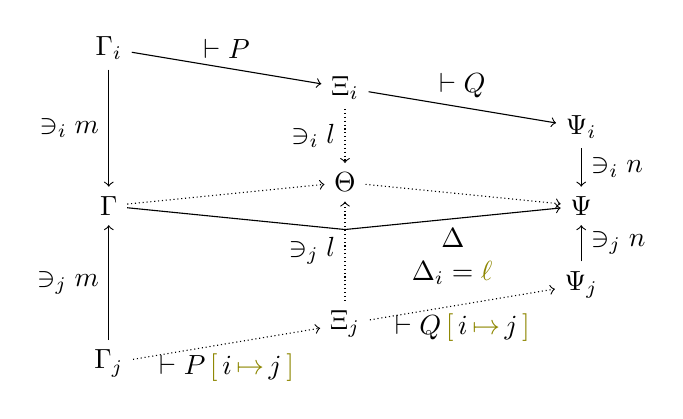
\begin{tikzpicture}
      \node (gamma-i) at (0,4)   {$\Gamma_i$};
      \node (gamma-m) at (0,2)   {$\Gamma$};
      \node (gamma-j) at (0,0)   {$\Gamma_j$};
      \node (xi-i)    at (3,3.5) {$\Xi_i$};
      \node (theta)   at (3,2.3) {$\Theta$};
      \node (delta-m) at (3,1.7) {};
      \node (xi-j)    at (3,0.5) {$\Xi_j$};
      \node (psi-i)   at (6,3)   {$\Psi_i$};
      \node (psi-m)   at (6,2)   {$\Psi$};
      \node (psi-j)   at (6,1)   {$\Psi_j$};

      \draw[-]  (gamma-m) -- (delta-m.center);
      \draw[->] (delta-m.center) -- node[align=center,below] {$\Delta$\\$\Delta_i = \lz$}(psi-m);

      \draw[->,densely dotted] (gamma-m) -- (theta);
      \draw[->,densely dotted] (theta) -- (psi-m);
      
      \draw[->] (gamma-i) -- node[left] {$\ni_i m$} (gamma-m);
      \draw[->] (gamma-j) -- node[left] {$\ni_j m$} (gamma-m);
      \draw[->] (psi-i) -- node[right] {$\ni_i n$} (psi-m);
      \draw[->] (psi-j) -- node[right] {$\ni_j n$} (psi-m);

      \draw[->] (gamma-i) -- node[above] {$\vdash P$} (xi-i);
      \draw[->] (xi-i) -- node[above] {$\vdash Q$} (psi-i);
      \draw[->,densely dotted] (gamma-j) -- node[below] {$\vdash \subst{P}{j}{i}$} (xi-j);
      \draw[->,densely dotted] (xi-j) -- node[below] {$\vdash \subst{Q}{j}{i}$} (psi-j);
      \draw[->,densely dotted] (xi-i) -- node[left] {$\ni_i l$} (theta);
      \draw[->,densely dotted] (xi-j) -- node[left] {$\ni_j l$} (theta);
    \end{tikzpicture}
    \caption{
      Diagrammatic representation of the $\comp{}{}$ case for renaming.
      Continuous lines represent known facts, dotted lines proof obligations.
    }
    \label{fig:subst}
\end{figure}

\begin{figure}[h]
    \centering
    \begin{tikzpicture}
      \node (gamma-i) at (0,2)   {};
      \node (gamma-m) at (0,1)   {};
      \node (gamma-j) at (0,0)   {};
      \node (xi-i)    at (2,3)   {};
      \node (xi-m)    at (2,2) {};
      \node (xi-j)    at (2,1)   {};
      \node (psi-m)   at (4,2) {};

      \draw[->] (gamma-i) -- (xi-j);
      \draw[->] (gamma-m) -- (xi-j);
      \draw[->,densely dotted] (gamma-j) -- (xi-j);
      \draw[->] (gamma-i) -- (gamma-m);
      \draw[->] (gamma-j) -- (gamma-m);
      \draw[->] (xi-i)    -- (xi-m);
      \draw[->] (xi-j)    -- (xi-m);
      \draw[->] (xi-i)    -- (psi-m);
      \draw[->] (xi-m)    -- (psi-m);
      \draw[->,densely dotted] (xi-j)    -- (psi-m);
    \end{tikzpicture}
    \caption{
      Alternative approach without arrows $\ni_i n$ and $\ni_j n$.
      This approach makes composing typing derivations before and after renaming more difficult.
    }
    \label{fig:subst-alternative}
\end{figure}

\begin{nitheorem}[Renaming]
  \label{thm:renaming}
  Let $P$ be well typed in $\types{\gamma \comma t}{\Gamma \comma m}{P}{\Psi \comma \lz}$.
  Let $\contains{\gamma}{\Psi}{j}{t}{m}{\Xi}$.
  Then, we can rename the variable references to $\constr{0}$ in $P$ with $\suc j$ so that the result is well typed in $\types{\gamma \comma t}{\Gamma \comma m}{\subst{P}{\suc j}{\constr{0}}}{\Xi \comma m}$.
\end{nitheorem}
\begin{proof}[Proof (Sketch)]
  We use framing to derive $\contains{\gamma}{\Gamma}{j}{t}{m}{\Theta}$ and $\types{\gamma \comma t}{\Theta \comma m}{P}{\Xi \comma \lz}$ for some $\Theta$.
  Then, we use these to apply \autoref{thm:renaming-generalization}.
\end{proof}

%%%%%%%%%%%%%%%%%%%%%%%%%%%%%%%%%%%%%%%%%%%%%%%%%%%%%%%%%%%%%%%%%%% 

% \begin{note}
  We use $\containsusage{\Gamma}{i}{x}{\Delta}$ to stand for $\contains{\gamma}{\Gamma}{i}{t}{x}{\Delta}$ for some $\gamma$ and $t$.
% \end{note}

\subparagraph*{Subject Reduction}
states that if $P$ is well typed and it reduces to $Q$, then $Q$ is well typed.
In the \picalc{} we distinguish between a reduction $P \reduce{\constr{internal}} Q$ on a channel internal to $P$, and a reduction $P \reduce{\constr{external} \; i} Q$ on a channel $i$ external to $P$ (refer to \autoref{operational-semantics}).

\begin{nitheorem}[Subject reduction]
  \label{thm:subject-reduction}
  Let $P$ be well typed in $\types{\gamma}{\Gamma}{P}{\Xi}$ and reduce such that $P \reduce{c} Q$.
  \begin{itemize}
    \item If $c$ is $\constr{internal}$, then $\types{\gamma}{\Gamma}{Q}{\Xi}$.
    \item If $c$ is $\constr{external} \; i$ and $\containsusage{\Gamma}{i}{\lio}{\Delta}$, then $\types{\gamma}{\Delta}{Q}{\Xi}$.
  \end{itemize}
\end{nitheorem}

\begin{proof}[Proof (Sketch)]
  By induction on $P \reduce{c} Q$.
  \hfill{}\\
  \begin{itemize}
    \item
    Case $\constr{comm}$: we apply framing (\autoref{thm:framing}) (to rearrange the assumptions), renaming (\autoref{thm:renaming}) and strengthening (\autoref{thm:strengthening}).
  
    \item
    Case $\constr{par}$: by induction on the process that is being reduced.

    \item
    Case $\constr{res}$: case split on channel $c$:
    if $\constr{internal}$ proceed inductively;
    if $\constr{external}\; \constr{0}$ (i.e. the channel introduced by scope restriction) use \autoref{lm:comm-capable} to subtract $\lio$ from the channel's usage annotation and proceed inductively;
    if $\constr{external}\; (\suc i)$ proceed inductively.

    \item
    Case $\constr{struct}$: we apply subject congruence (\autoref{thm:subject-congruence}) and proceed inductively. \qedhere
  \end{itemize}
\end{proof}

%%%%%%%%%%%%%%%%%%%%%%%%%%%%%%%%%%%%%%%%%%%%%%%%%%%%%%%%%%%%%%%%%%% 
\section{Conclusion, Related and Future Work}

Allais \cite{Allais2018a} uses leftover typing to mechanise in Agda a bidirectional type system for the linear \lambdacalc{}.
He proves type preservation and provides a decision procedure for type checking and type inference.
In this paper, we follow Allais \cite{Allais2018a} and apply leftover typing to the \picalc{}.
We give a more general usage algebra, leading to linear, graded and shared type systems.
Drawing from quantitative type theory (by McBride and Atkey \cite{McBride2016, Atkey2018}), in our work, we too are able to talk about fully consumed resources --- e.g., we can transmit over a channel $\lz$ multiplicities of a fully exhausted channel.
%
In their recent paper (unpublished at the time of writing), Ciccone and Padovani mechanise a dependently-typed linear \picalc{} in Agda \cite{Ciccone}.
They do so by defining an intrinsicly-typed calculus, which allows them to leverage Agda to provide a dependently-typed interpretation of messages.
Contexts contain not only types, but also the messages that inhabit their corresponding interpretation in Agda.
To avoid linearity violations, channel types as interpreted as unit types --- and therefore only present in the context in the object language.
This approach allows them to encode message predicates, branching, and variable-length conversations, as message input is modelled as dependent function abstraction in Agda.
They use the concrete set of multiplicities $0$, $1$, $\omega$, define a partial algebra on contexts and require extrinsic proofs of context split.
%
Orchard et al. introduce Granule \cite{Orchard}, a fully-fledged functional language with graded modal types, linear types, indexed types and polymorphism.
Modalities include exact usages, security levels and intervals; resource algebras are pre-ordered semirings with partial addition.
They provide bidirectional typing rules, and show the type safety of their semantics.

Recent years have seen an increase in the efforts to mechanise resource-aware process algebras.
One of the earliest works is the mechanisation of the linear \picalc{} in Isabelle/HOL by Gay \cite{Gay2001}.
Gay encodes the \picalc{} with linear and shared types using de Bruijn indices, a reduction relation and a type system posterior to the syntax.
However, in his work context splits are extrinsic, and used multiplicities erased from context.
We make context splits intrinsic, preserve the ability to talk about used resources, and adopt a more general usage algebra: our framework integrates three different type systems into one.
%
The work by Goto et al. \cite{Goto2016a} is, to the best of our knowledge, the first formalisation of session types that includes a type safety proof (in Coq). 
The authors extend session types with polymorphism and pattern matching.
They use a locally-nameless encoding for variable references, a syntax prior to types, and an LTS semantics that encodes session-typed processes into the \picalc{}.
Their type system uses reordering of contexts and extrinsic context splits. 
%
Castro et al. \cite{Castro2020} provide tooling for locally-nameless representations of process calculi in Coq  --- in Coq de Bruijn indices are not as popular as in Agda or Idris because dependent pattern matching is far from straightforward.
As a use-case, they use their tool to help automate proofs of subject reduction for a type system with session types.
%
Taking an intrinsic approach to typing, Thiemann formalises in Agda the MicroSession (minimal GV \cite{Gay2010}) calculus with support for recursion and subtyping \cite{Thiemann2019}.
Context splits are still given extrinsically, and exhausted resources are removed from typing contexts altogether.
The semantics are given as an intrinsically typed CEK machine with a global context of session-typed channels.
%
Most recently, Rouvoet et al. provide an intrinsic type system for a \lambdacalc{} with session types \cite{Rouvoet2020}.
They use proof relevant separation logic and a notion of a supply and demand \emph{market} to make context splits transparent to the user.
Their separation logic is based on a partial commutative monoid that need not be deterministic nor cancellative.
Their typing rules preserve the balance between supply and demand, and are extremely elegant.
They distill their typing rules even further by modelling the supply and demand market as a state monad.
%
Based on contextual type theory \cite{Pientkaa, Pientka}, LINCX \cite{Georges2017} extends the linear logical framework LLF \cite{Cervesato1996} by internalising the notion of bindings and contexts.
The result is a meta-theory in which HOAS encodings with both linear and dependent types can be described.
The developer obtains for free an equational theory of substitution and decidable typechecking without having to encode context splits within the object language.

Further work on mechanising the \picalc{} \cite{Henry-Gerard1999, Honsell2001a, Bengtson2013, Despeyroux2000, Affeldt2008}, focuses on non-linear variations, whereas we present a range of linear, graded and shared types.

%%%%%%%%%%%%%%%%%%%%%%%%%%%%%%%%%%%%%%%%%%%%%%%%%%%%%%%%%%%%%%%%%%%
To conclude, in this paper we provide a well scoped syntax and a semantics for the \picalc{}, extrinsically define a type system on top of the syntax capable of handling linear, graded and shared types under the same unified framework and show that reduction preserves the well-typedness of processes.
We avoid the need for extrinsic context splits by defining a type system based on leftover typing \cite{Allais2018a}, which is defined here for the first time for the \picalc{}.
As a result, theorems like framing, weakening and strengthening can now we stated for the linear \picalc{}.
Our work is fully mechanised in around 1500 lines of code in Agda%
\begin{anonsuppress}
\cite{Zalakain2020Agda}
\end{anonsuppress}
.
%
As future work, we intend to prove further properties of our type system, such as that reduction preserves the balancing of channels.
We intend to add support for products, sum types and recursion to both our syntax and our type system.
Orthogonally, making our typing rules bidirectional would allow us to provide a decision procedure for type checking processes in a given set of algebras.
Furthermore, it might also be worth identifying correspondences between our usage algebra and particular state machines.
Finally, we will use our \picalc{} with leftovers as an underlying framework on top of which we can implement session types and other advanced type theories.

\bibliographystyle{plainurl}
\bibliography{paper}

%%
\appendix
%% Appendix
\section{Structural Congruence}
\label{app:struct}

Structural congruence is a congruent equivalence relation.
As such, rewrites can happen anywhere inside a process, and are closed under reflexivity, symmetry and transitivity as shown by the first row of \autoref{fig:struct-cong1}.
The rest of the rules defines structural congruence under a context $\mathcal{C}[\cdot]$ \cite{Sangio01}, respectively restriction, composition, input and output.

\begin{figure}[h]
  \begin{mathpar}
    \datatype
    { }
    {\Rec : \Set}
    \; \textsc{Rec}
  
    \inferrule
    { }
    {\constr{zero} : \Rec}
    
    \inferrule
    {r : \Rec}
    {\constr{one} \; r : \Rec}
  
    \inferrule
    {r \; s : \Rec}
    {\constr{two} \; r \; s : \Rec}
    
    \datatype
    {P \, Q : \Process_n \\ r : \Rec}
    {P \eq{r} Q : \Set}
    \; \textsc{Equals}
  
    \inferrule
    {eq : P \eqeq Q}
    {\constr{struct} \; eq : P \eq{\constr{zero}} Q}
  
    \inferrule
    {eq : P \eq{r} P'}
    {\constr{cong-scope} \; eq : \new P \eq{\constr{one} \; r} \new P'}
  
    \inferrule
    {eq : P \eq{r} P'}
    {\constr{cong-comp} \; eq : \comp{P}{Q} \eq{\constr{one} \; r} \comp{P'}{Q}}
  
    \inferrule
    {eq : P \eq{r} P'}
    {\constr{cong-recv} \; eq : \recv{x}P \eq{\constr{one} \; r} \recv{x}P'}
  
    \inferrule
    {eq : P \eq{r} P'}
    {\constr{cong-send} \; eq : \send{x}{y}P \eq{\constr{one} \; r} \send{x}{y}P'}
  
    \inferrule
    { }
    {\constr{refl} : P \eq{\constr{zero}} P}
  
    \inferrule
    {eq : P \eq{r} Q}
    {\constr{sym} \; eq : Q \eq{\constr{one} \; r} P}
  
    \inferrule
    {eq_1 : P \eq{r} Q \\ \; eq_2 : Q \eq{s} R}
    {\constr{trans} \; eq_1 \; eq_2 : P \eq{\constr{two} \; r \; s} R}
  \end{mathpar}
  \caption{Structural rewriting rules lifted to a congruent equivalence relation indexed by a recursion tree.}
  \label{fig:struct-cong1}
  \end{figure}

In the transitivity rule, we must show that if $P$ is structurally congruent to $Q$ and $Q$ is to $R$, and $P$ is well-typed, then so is $R$.
To do so, we need to proceed by induction and first get a proof of the well-typedness of $Q$, then use that to reach $R$.
To show the typechecker that the doubly recursive call terminates we index the equivalence relation $=$ by a type $\Rec$ that models the structure of the recursion.

\section{Usage Algebra}
\label{app:usage-algebra}

\todo{we haven't introduced the forall and implicit syntax}
\todo{introduce DEC and exists}

Our usage algebra is a ternary relation $\op{x}{y}{z}$ that is \emph{partial}, \emph{functional}, \emph{cancelative}, \emph{associtive}, and \emph{commutative}.
It has a \emph{neutral element} $\zero$ that is absorbed on either side, and that is also \emph{minimal}.
It has an element $\one$ that is used to count inputs and outputs.
These algebraic laws are defined as a record $\Quantifier_C$ on a carrier set $C$ in \autoref{fig:multiplicities}.
We use a terniary relation to model the partial monoidal operation.
We then encapsulate a set carriers and their algebras in \autoref{fig:indexed-multiplicities}.

\begin{figure}[h]
\begin{equation}
\begin{aligned}
  &\zero                  &:{} &                      &        & C \\
  &\one                   &:{} &                      &        & C \\
  &\op{\_}{\_}{\_}        &:{} &                      &        & C \to C \to C \to \Set \\
  &\func{\cdot-compute}  &:{} &\forall y z           & \to \; & \type{DEC} \; (\type{\exists} x . \; (\op{x}{y}{z})) \\
  &\func{\cdot-unique}   &:{} &\forall \{x x' y z\}  & \to \; & \op{x'}{y}{z} \to \op{x}{y}{z} \to x' \equiv x \\
  &\func{\cdot-unique^l} &:{} &\forall \{x y y' z\}  & \to \; & \op{x}{y'}{z} \to \op{x}{y}{z} \to y' \equiv y \\
  &\func{0\cdot-min^l}   &:{} &\forall \{y z\}       & \to \; & \op{\zero}{y}{z} \to y \equiv \zero \\
  &\func{\cdot-id^l}     &:{} &\forall \{x\}         & \to \; & \op{x}{\zero}{x} \\
  &\func{\cdot-comm}     &:{} &\forall \{x y z\}     & \to \; & \op{x}{y}{z} \to \op{x}{z}{y} \\
  &\func{\cdot-assoc}    &:{} &\forall \{x y z u v\} & \to \; & \op{x}{y}{z} \to \op{y}{u}{v} \to \type{\exists} w . \; (\op{x}{u}{w} \times \op{w}{v}{z})
\end{aligned}
\end{equation}
\caption{Quantifier algebra $\Quantifier_C$ algebra on a partial commutative monoid.}
\label{fig:multiplicities}
\end{figure}

\begin{figure}[h]
  \begin{equation}
    \begin{split}
      &\func{IDX}          &:{} &\Set \\
      &\func{\exists IDX}  &:{} &\func{IDX} \\
      &\func{USAGE}        &:{} &\func{IDX} \to \Set \\
      &\func{QUANTIFIERS}  &:{} &(i : \func{IDX}) \to \Quantifier_{\func{USAGE}_i}
    \end{split}
  \end{equation}
  \caption{Indexed set of usage algebras.}
  \label{fig:indexed-multiplicities}
\end{figure}

\section{Lemmas}
\label{app:lemmas}

\begin{nilemma}
  \label{lm:subst-unused}
  For every variables $i$ and $j$, if $i \not\equiv j$ then $\Unused_i (\subst{P}{j}{i})$.
\end{nilemma}
\begin{proof}
  By structural induction on \textsc{Process} and \textsc{Var}.
\end{proof}

\begin{nilemma}
  \label{lm:lower-lift}
  The function $\func{lower}_i \; P \; uP$ has an inverse $\func{lift}_i \; P$ that increments every $\textsc{Var}$ greater than or equal to $i$, such that $\func{lift}_i \; (\func{lower}_i \; P \; uP) \equiv P$.
\end{nilemma}
\begin{proof}
  By structural induction on \textsc{Process} and \textsc{Var}.
\end{proof}

\begin{nilemma}
  \label{lm:swap-swap}
  The function $\func{swap}_i \; P$ is its own inverse: $\func{swap}_i \; (\func{swap}_i \; P) \equiv P$.
\end{nilemma}
\begin{proof}
  By structural induction on \textsc{Process} and \textsc{Var}.
\end{proof}

\begin{nilemma}
  \label{lm:types-unused}
  For all well-typed processes $\types{\gamma}{\Gamma}{P}{\Xi}$, if the variable $i$ is unused within $P$, then $\Gamma$ at $i$ is equivalent to $\Xi$ at $i$.
\end{nilemma}
\begin{proof}
  By induction on \textsc{Process} and \textsc{Var}.
\end{proof}

\begin{nilemma}
  \label{lm:types-op}
  For all well-typed processes $\types{\gamma}{\Gamma}{P}{\Xi}$, there exists some $\Delta$ such that $\opctx{\Gamma}{\Delta}{\Xi}$.
\end{nilemma}
\begin{proof}
  By induction on \textsc{Process} and \textsc{Var}.
\end{proof}

\begin{nilemma}
  \label{lm:comm-capable}
  Every input usage context $\Gamma$ of a well-typed process $\types{\gamma}{\Gamma}{P}{\Delta}$ that reduces by communicating on a channel external to it (that is, $P \reduce{\constr{external} \; i} Q$ for some $Q$) has a multiplicity of at least $\lio$ at index $i$.
\end{nilemma}

\begin{proof}
  By induction on the reduction derivation $P \reduce{\constr{external \; i}}Q$.
\end{proof}
\end{document}
